\chapter{Test Journal for Sensor Variances}
\label{sc:variances}

\section{Objective}
The objective is to determine the measurement variances on the sensors
that can be used for state estimation of the ship for control
purposes. This is the \ac{IMU} and \ac{GPS} measurements.

\section{Theory}
The variance is a key constant that state estimators rely on to weigh
how much it should trust a measurement, hence the value must be known.

The variance is the standard deviation squared, and can be determined
from a time series of measurements from the sensors. The variance for
a discrete random variable can be calculated as:
\begin{align}
	\mathrm{Var}(X) = \frac{1}{n} \sum_{i=1}^n (x_i - \mu) ^2
\end{align}
where the expected value $\mu$ is for example
\begin{align}
	\mu = \frac{1}{n} \sum_{i=1}^n x_i.
\end{align}

\section{Tools}
\begin{enumerate}
	\item One AAUSHIP with sensors and \ac{HLI} to log the data.
	\item The data was processed in \MATLAB\ with the command
		\texttt{var()}.
\end{enumerate}

\section{Results}

The computed vales is;
\begin{alignat*}{3}
&^\text{IMU}\sigma_{m_x}^2 = 1.0415e^{-6},
\quad& &
^\text{IMU}\sigma_{m_y}^2 = 544.2176e^{-9},
\quad& &
^\text{IMU}\sigma_{m_z}^2 = 419.2507e^{-9},
\\ \nonumber
&^\text{IMU}\sigma_{g_x}^2 = 94.0726e^{-3},
\quad& &
^\text{IMU}\sigma_{g_y}^2 = 28.1434e^{-3},
\quad& &
^\text{IMU}\sigma_{g_z}^2 = 99.3437e^{-3},
\\ \nonumber
&^\text{IMU}\sigma_{a_x}^2 = 285.4267e^{-6},
\quad& &
^\text{IMU}\sigma_{a_y}^2 = 264.4893e^{-6},
\quad& &
^\text{IMU}\sigma_{a_z}^2 = 317.1120e^{-6}.
\end{alignat*}

         

\begin{figure}[htpb]
	\centering
	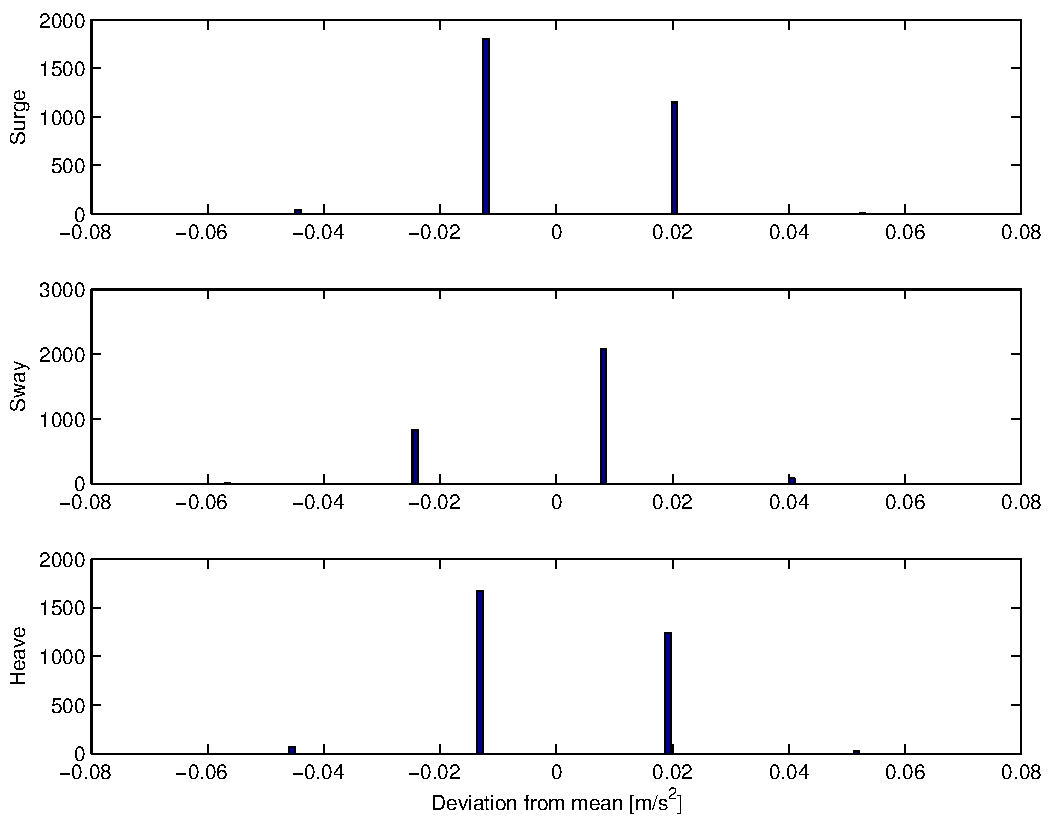
\includegraphics[width=\textwidth]{pdf/acclhist3000}
	\caption{Histogram of the accelerometer. 100 bins. 3000 samples.}
	\label{fig:acclhist3000}
\end{figure}

\begin{figure}[htpb]
	\centering
	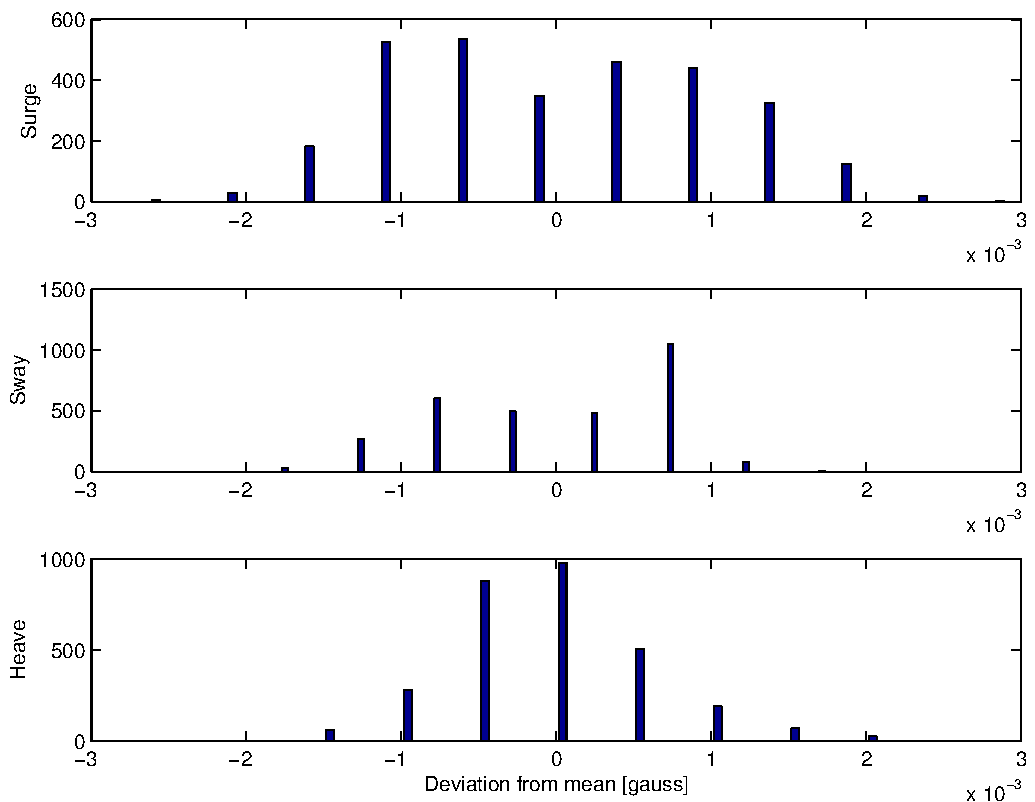
\includegraphics[width=\textwidth]{pdf/magnhist3000}
	\caption{Histogram of the magnetometer. 100 bins. 3000 samples.}
	\label{fig:magnhist3000}
\end{figure}

\begin{figure}[htpb]
	\centering
	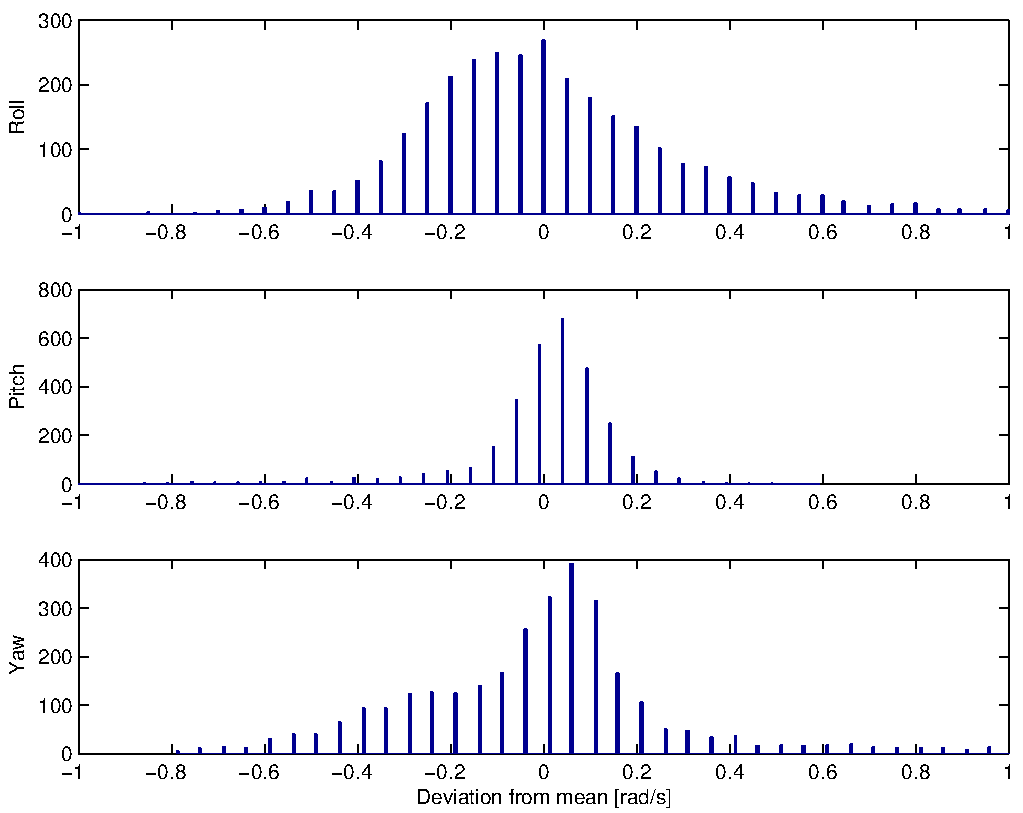
\includegraphics[width=\textwidth]{pdf/gyrohist3000}
	\caption{Histogram of the gyrometer. 1000 bins. 3000 samples.}
	\label{fig:gyrohist3000}
\end{figure}

\begin{figure}[htpb]
	\centering
	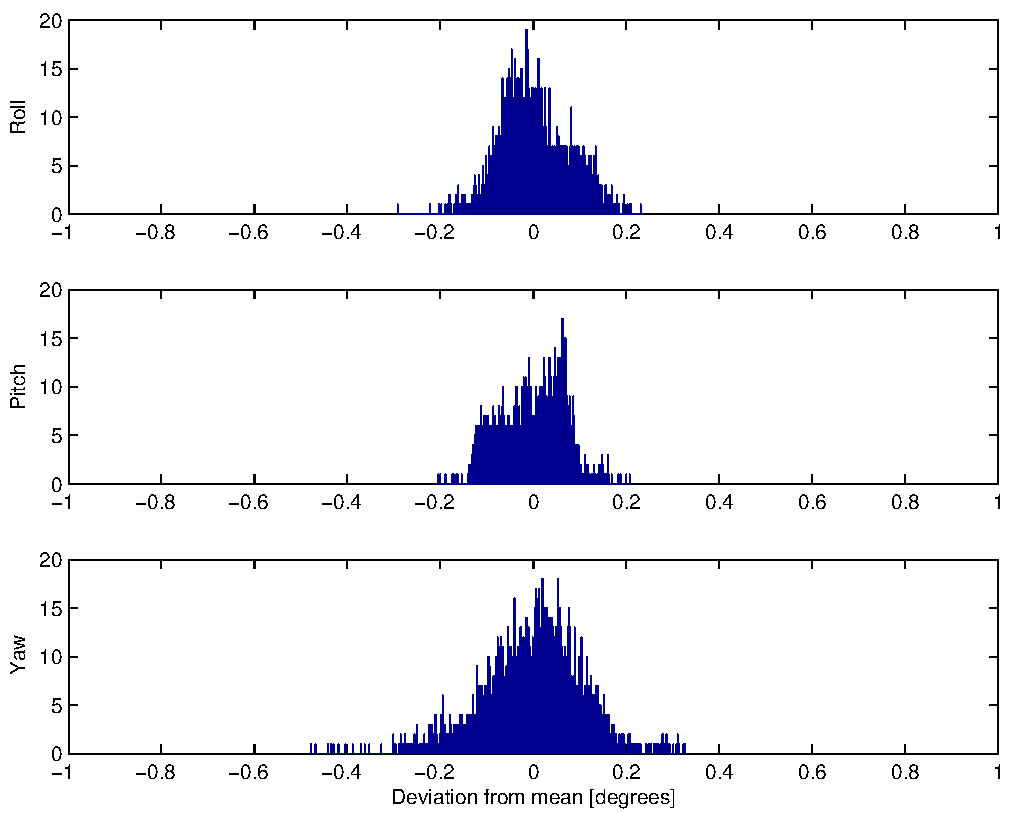
\includegraphics[width=\textwidth]{pdf/mahonyhist3000}
	\caption{Histogram of the estimated attitude with the Mahony filter
	with the filter constants; sample time of 1/20 s, $K_p = 8.8$, $K_i
= 0.5$. 1000 bins. 3000 samples.}
	\label{fig:mahonyhist3000}
\end{figure}


\section{Discussion and Conclusion}
It is seen on the histogram plots that the shapes is not beautifully gaussian shaped. This can be because there is some slow bias drift on the sensor and the fact that the the noise is around a few samples. Especially for the accelerometer on figure~\vref{fig:acclhist3000} where it is only four samples and most on the middle two.

Variances of the time series for all plots was determined and presented in the results section.
